\documentclass[a4paper]{IEEEtran}

% Ein paar hilfreiche Pakete
\usepackage[utf8]{inputenc}
\usepackage[ngerman]{babel}
\usepackage{graphicx}
\usepackage{amsmath}
\usepackage{amssymb}
\usepackage{mathtools}
\usepackage{subcaption}
\usepackage{hyperref}

% Nummeriere Formel nur, wenn sie auch referenziert wird
\mathtoolsset{showonlyrefs}

% Header
\markboth{Seminar SS 2020 Moderne Methoden der Informationsverarbeitung}{}

% Hier den Titel des eigenen Seminars eintragen
\title{Thema des Seminars}

% Hier deinen eigenen Namen
\author{Vorname~Nachname}


\begin{document}

% Erzeugt die Überschrift
\maketitle

% Zusammenfassung
\begin{abstract}
Die Ausarbeitung beginnt mit einer kurzen Zusammenfassung.
\end{abstract}

% Erster Abschnitt
\section{Introduction}

Hier beginnt der Text...

\section{Ein paar Hinweise}

Vor eine Subsection gehören immer noch ein paar einleitende Worte!

\subsection{Absätze, etc.}

Ein neuer Absatz sollte nicht durch einen Zeilenumbruchs-Befehl, sondern durch eine Leerzeile im Code erzeugt werden.

Das hier ist richtig.
\\ Das hier nicht.

\subsection{Formeln}

So können Formeln gesetzt und referenziert werden:
\begin{equation}
    a = b + c \,.
    \label{eq:name}
\end{equation}
Laut \eqref{eq:name} ist $a=b+c$. Formeln sind Teil des Fließtextes und sollten deshalb korrekt mit Punkten und Kommata interpunktiert werden.  Das \texttt{\textbackslash,} fügt dabei einen kleinen Abstand zwischen Formel und Interpunktion ein.

Mehrzeiliger Formelsatz mit der \emph{split} Umgebung innerhalb der \emph{equation} Umgebung:
\begin{equation}
    \begin{split}
        % \\ für Zeilenumbruch
        % an & wird ausgerichtet
        a      &= b + c \,, \\
        a_{ij} &= b_{ij} + c_{ij} \,.
    \end{split}
\end{equation}

Funktionen sollen in Formeln \emph{nicht} mit mathematischer Schrift gesetzt werden.
Dazu gibt es in LaTeX für fast alle Funktionen schon Makros, z.B. 
\begin{align}
    y = \sin(x)\,,
\end{align}
nicht 
\begin{align}
    y = sin(x)
\end{align}
benutzen. Für nicht vorhandene Funktionen kann \emph{operatorname} eingesetzt werden:
\begin{equation}
    y = \operatorname{spur}(X) \,.
\end{equation}

\subsection{Bilder}

So werden Bilder eingebunden (als pdf, jpg oder png):

\begin{figure}[!h]
    \centering
    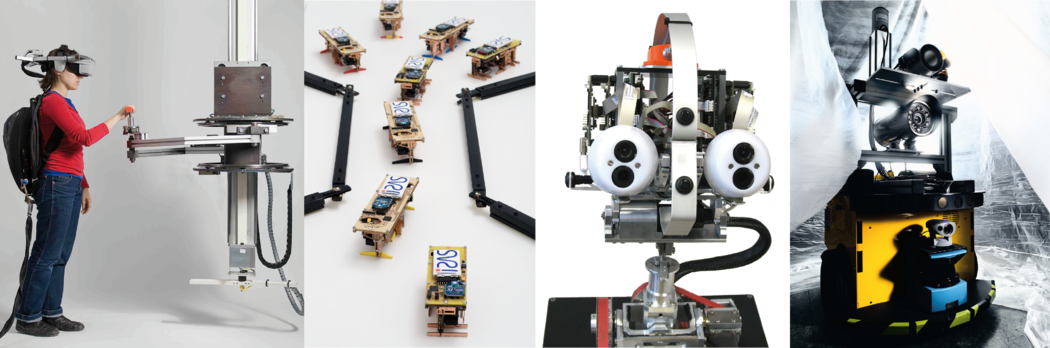
\includegraphics[width=0.48\textwidth]{Bild.png}
    \caption{Hier kommen weitere Erklärungen zum Bild.}
    \label{fig:bild}
\end{figure}

Auf diese Abbildung wird dann mit Abb. \ref{fig:bild} verwiesen.

\subsection{Zitate}

Immer korrekt zitieren \cite{yaakov_bar-shalom_estimation_2001}!

\subsection{LaTeX Hilfe}

Diese Website ist sehr nützlich:

\url{http://en.wikibooks.org/wiki/LaTeX}

\section{Zusammenfassung und Ausblick}


\begin{enumerate}
    \item State estimation in dynamic systems (e.g in robotic )
    \begin{enumerate}
        \item context about what estimation is wrt. to a system
        \item state is not directly observable and we need measurement in order to estimate the state
        \item noisy measurements
        \item linear and non-linear systems (e.g. Kalman Filter in linear case and Unscented Kalman Filter in non-linear)
    \end{enumerate}
    \item prediction and filtering steps in the estimation
    \item problems in estimation
    \begin{enumerate}
        \item closed form representation of the desired density function are most often not possible 
        (in non-linear case) $\rightarrow$ approximation of probability density
        \item storing all information and propagate it every time step is computational expensive $\rightarrow$ progressive
    \end{enumerate}
    \item Short overview of different methods that focuses on non-linear dynamic systems (state of the art)
    \begin{enumerate}
        \item Methods using ODE (track true density via ODE)
        \item Other methods
    \end{enumerate} 
    \item Give an outlook on the seminar objective (not quite sure). Either one ODE method and one other non-linear filter method
    or a different ODE methods
\end{enumerate}
Sources:
\cite{hanebeck2003}
\cite{huber2008a}
\cite{daum2005}
\cite{hagmar2011}

\begin{itemize}
    \item system and measurment quations (nonlinear mapping)
    \item specification of noise $\rightarrow$ white noise 
    \item First order markov process $$p(x_{k} \vert x_{0:k-1}) = p(x_{k} \vert x_{k-1})$$
    with $x_{0:k-1} := \{x_{0}, x_{1}, \dots, x_{k-1}\}$ 
    \item the general estimation process has two steps
    \begin{itemize}
        \item prediction or time update $\rightarrow$ prior probability density $p(x_{k+1} \vert y_{0:k}, u_{0:k})$
        \item filtering step or measurement update $\rightarrow$ posterior probability density $p(x_{k+1} \vert y_{0:k+1}, u_{0:k})$
        \item How are they computed and what does they mean
    \end{itemize}
    \item Progressive bayes
\end{itemize}
System and measurment equation:
\begin{equation}
    \begin{split}
        % \\ für Zeilenumbruch
        % an & wird ausgerichtet
        x_{k+1}  &= a_{k}(x_{k}, u_{k}, w_{k}) \,, \\
        y_{k}    &= h_{k}(x_{k}, v_{k}) \,.
    \end{split}
\end{equation}
Connection between prediction and filtering in sense of Bayes Theorem
\begin{equation}
    p(x_{k+1} \vert y_{0:k+1}, u_{0:k}) =  \frac{p(y_{k} \vert x_{k})p(x_{k+1} \vert y_{0:k}, u_{0:k})}{p(y_{k+1} \vert y_{0:k})}\,, \\
\end{equation}

Sources:
\cite{chen2003}
% Literaturverzeichnis in Literatur.bib
% (z.B. per Hand oder mit Zotero, Jabref, etc. editieren) 
\bibliographystyle{plain}
\bibliography{Literatur}
\end{document}
